  \subsection{Características de detección}

  Para la presente experiencia, se determina la respuesta en frecuencia, del conjunto 
  amplificador de frecuencia intermedia y el detector de frecuencia modulada del 
  receptor.

  En primer lugar, se debe configurar el osciloscopio de la siguiente forma: 
  controles de ganancia en posición media, y \textbf{modo X-Y}. Se necesita modificar 
  la amplitud de los canales varias veces durante la experiencia, por lo que 
  no es crítica la posición de éstas.

  Luego, se inyecta la salida del generador de barrido en la 
  antena del receptor, la cual inicialmente está seteada en $\mathbf{10,7~MHz}$.

  Para no desarmar el receptor, se toma la salida del mismo en el conector 
  de audífonos, a partir de éste punto, se debe tener en cuenta la influencia 
  del control del volumen en la medición.

  Finalmente, se configura la salida del generador como muestra la Tabla 
  \ref{tab:ControlesGenExp2}.

  \begin{table}[H] 
    \centering 
    \begin{tabular}[H]{c c c}\hline
      \textbf{Comando} & \textbf{Posición} & \textbf{Comentarios} \\  \hline  
          Mod.Select    &       Off         &     Sin modulación  \\  \hline
          Marker Size   &       Mínimo      &   El botón pulsado  \\  \hline
          Frec. Rang    &      B            &  Banda $6~MHz$ a $18~MHz$ \\  \hline
          Sweep Width   &   Posición media  &       -             \\  \hline
          Aten. por pasos &       1         &       -             \\  \hline
          Aten. fino    &   Posición media  &       -             \\  \hline
          Marker Freq.  &   $10,7MHz$       & Frec. Central de  FI \\  \hline
          Sep Freq.     & FM-IF ($10,7~MHz$) & Frec. Central de  FI \\  \hline
    \end{tabular}
    \caption{Controles del generador para Experimento 2.}
    \label{tab:ControlesGenExp2}
  \end{table}

    El esquema de conexiones que se debe implementar con los dispositivos antes mencionados, se puede observar en
    la Figura~\ref{fig:EsquemaConexiones}. 

    \begin{figure}[H]
      \centering
      \frame{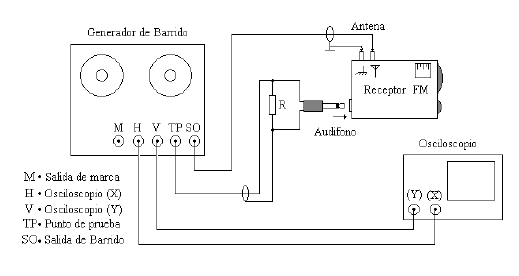
\includegraphics[width=0.6\textwidth]{Imagenes/ActividadPractica/CaracteristicasDeDeteccion/EsquemaConexiones.png}}
      \caption{Esquema de conexiones para las mediciones.}
      \label{fig:EsquemaConexiones}
    \end{figure}

    Luego, en la Figura~\ref{fig:InstrumentosParaFI} se encuentra la implementación del experimento. Además, a 
    modo de apreciar el funcionamiento del generador de barrido y marcas, en la Figura~\ref{fig:EspectroaFI} se 
    logra ver la respuesta en frecuencia junto con la marca.

    \begin{figure}[H]
      \centering
      \begin{subfigure}[ht]{0.48\textwidth}
        \frame{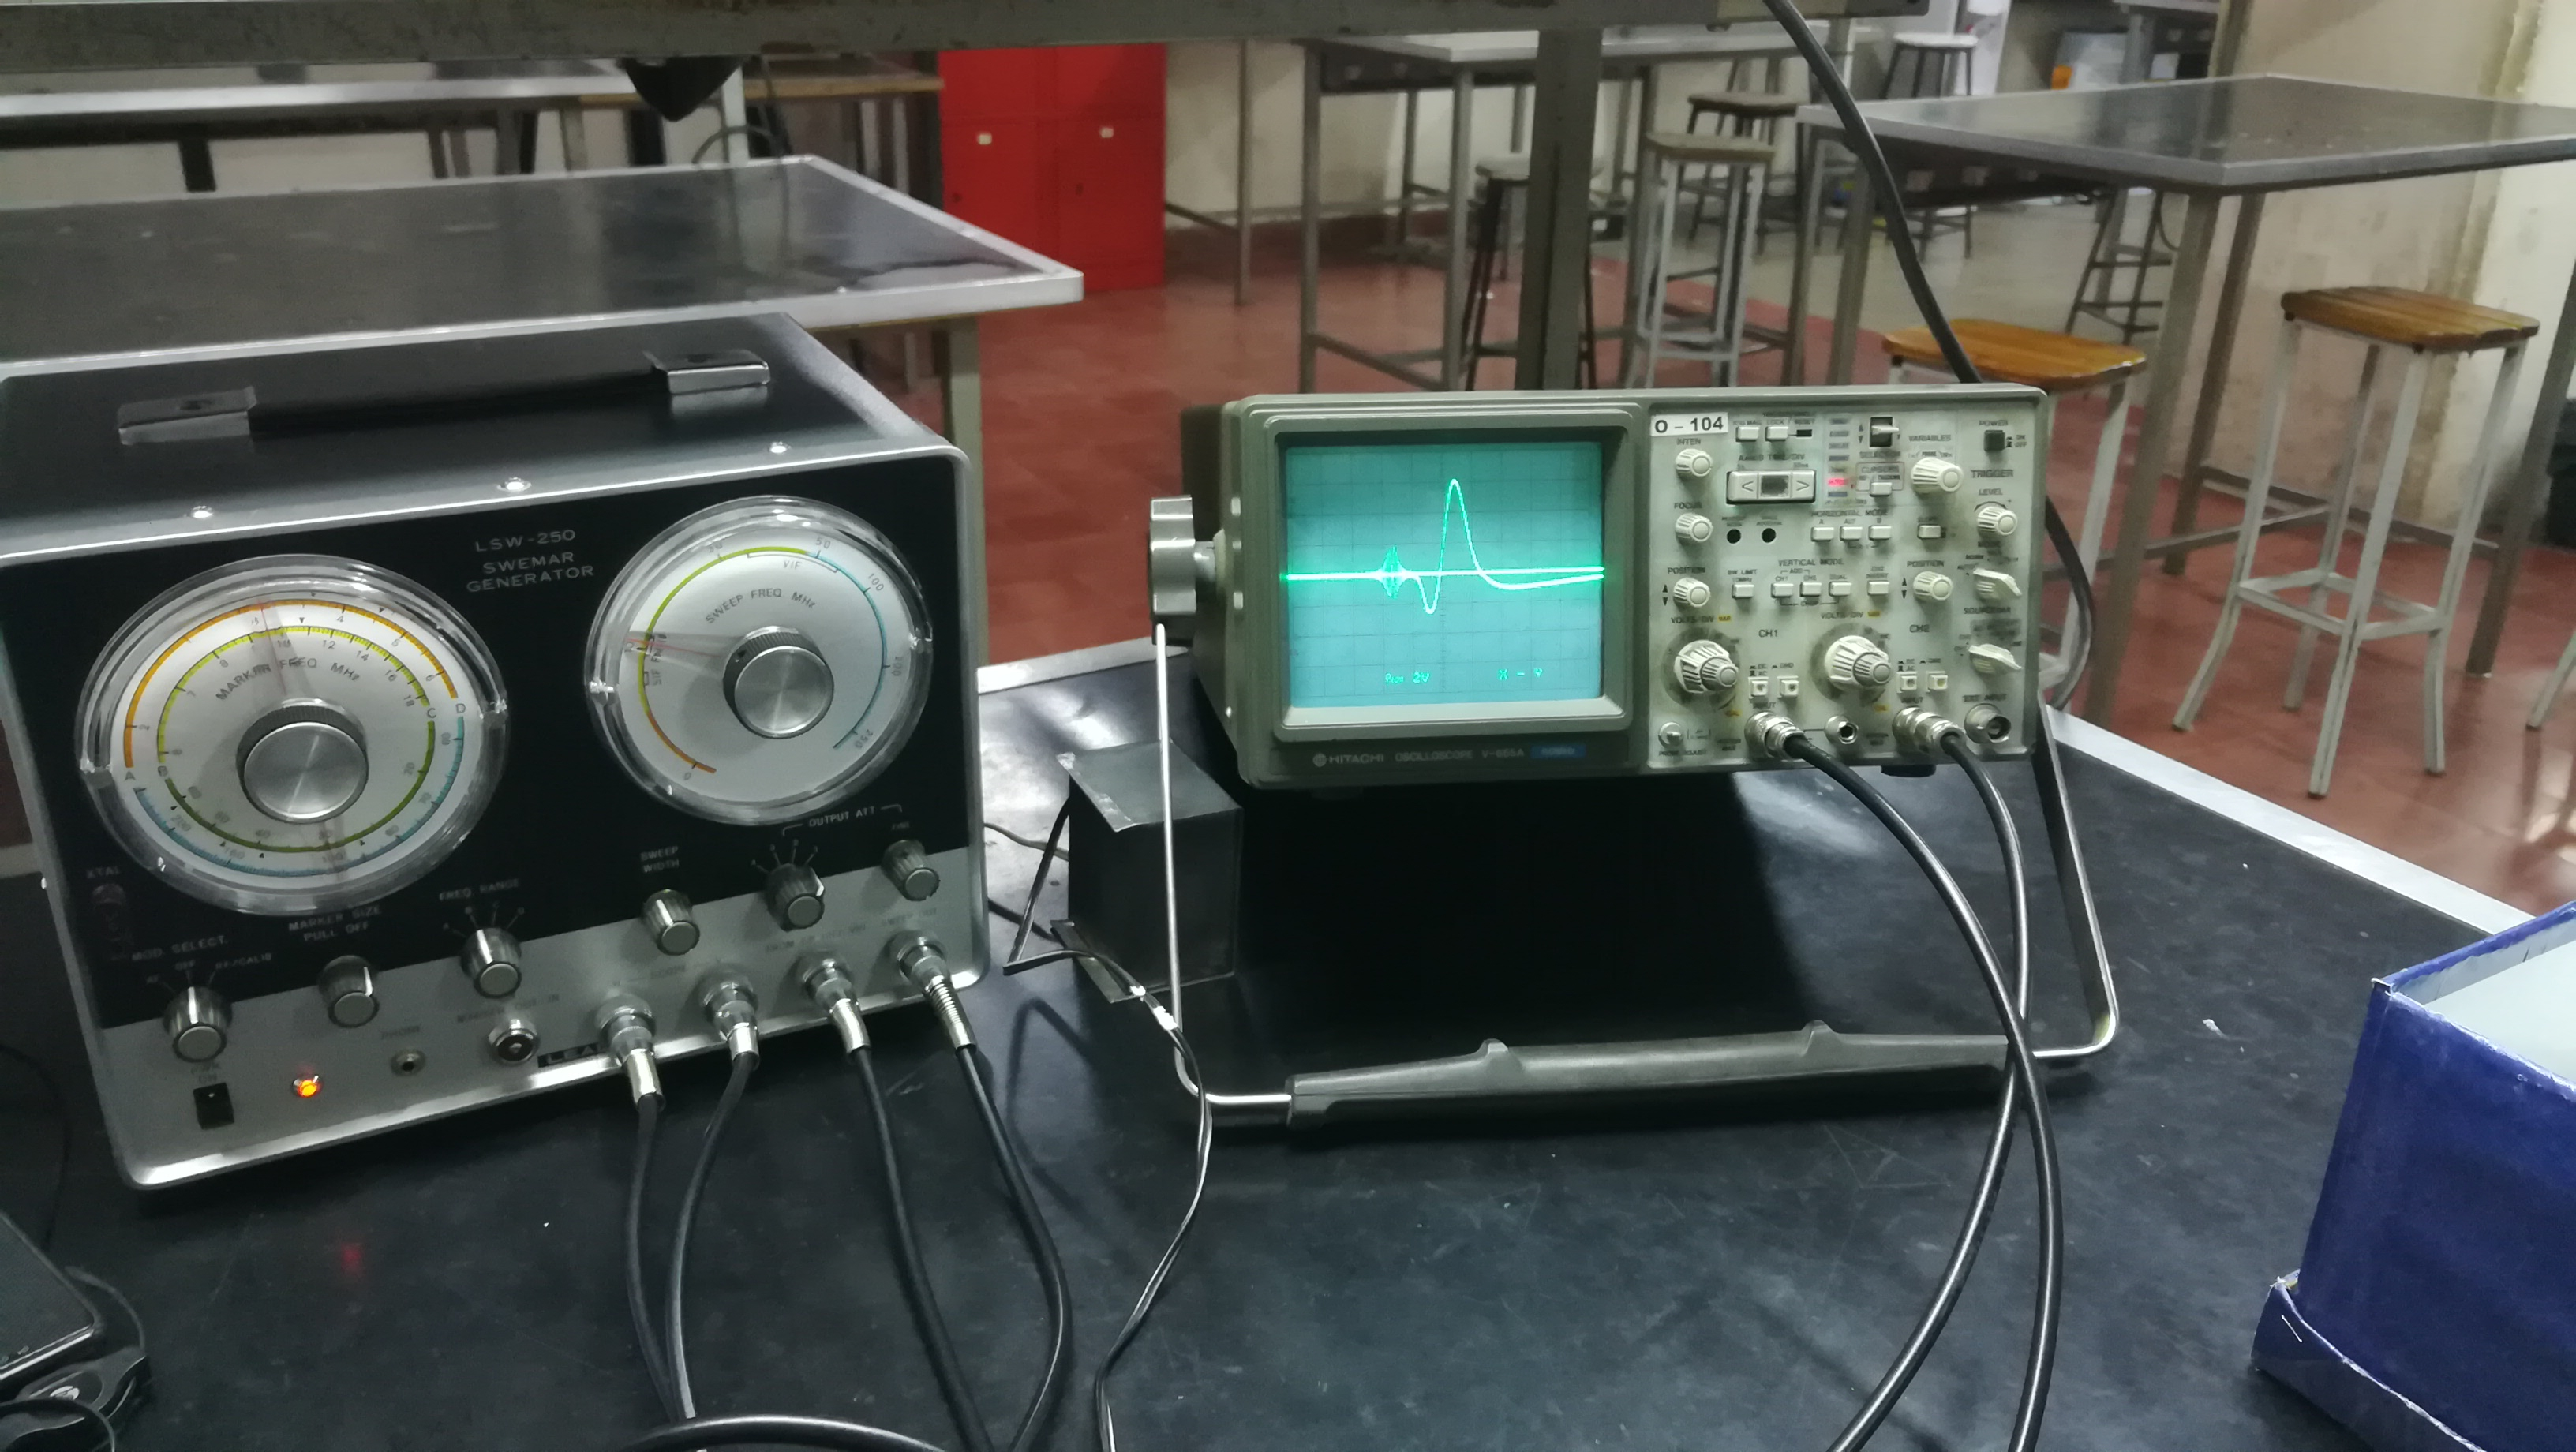
\includegraphics[width=\textwidth]{Imagenes/ActividadPractica/CaracteristicasDeDeteccion/Exp2.1_AmpliFI_InstrumentosConMarcaAIzquierda.jpg}}
        \caption{Disposición de instrumentos.}
        \label{fig:InstrumentosParaFI}
      \end{subfigure}
      \hfill 
      \begin{subfigure}[ht]{0.48\textwidth}
        \frame{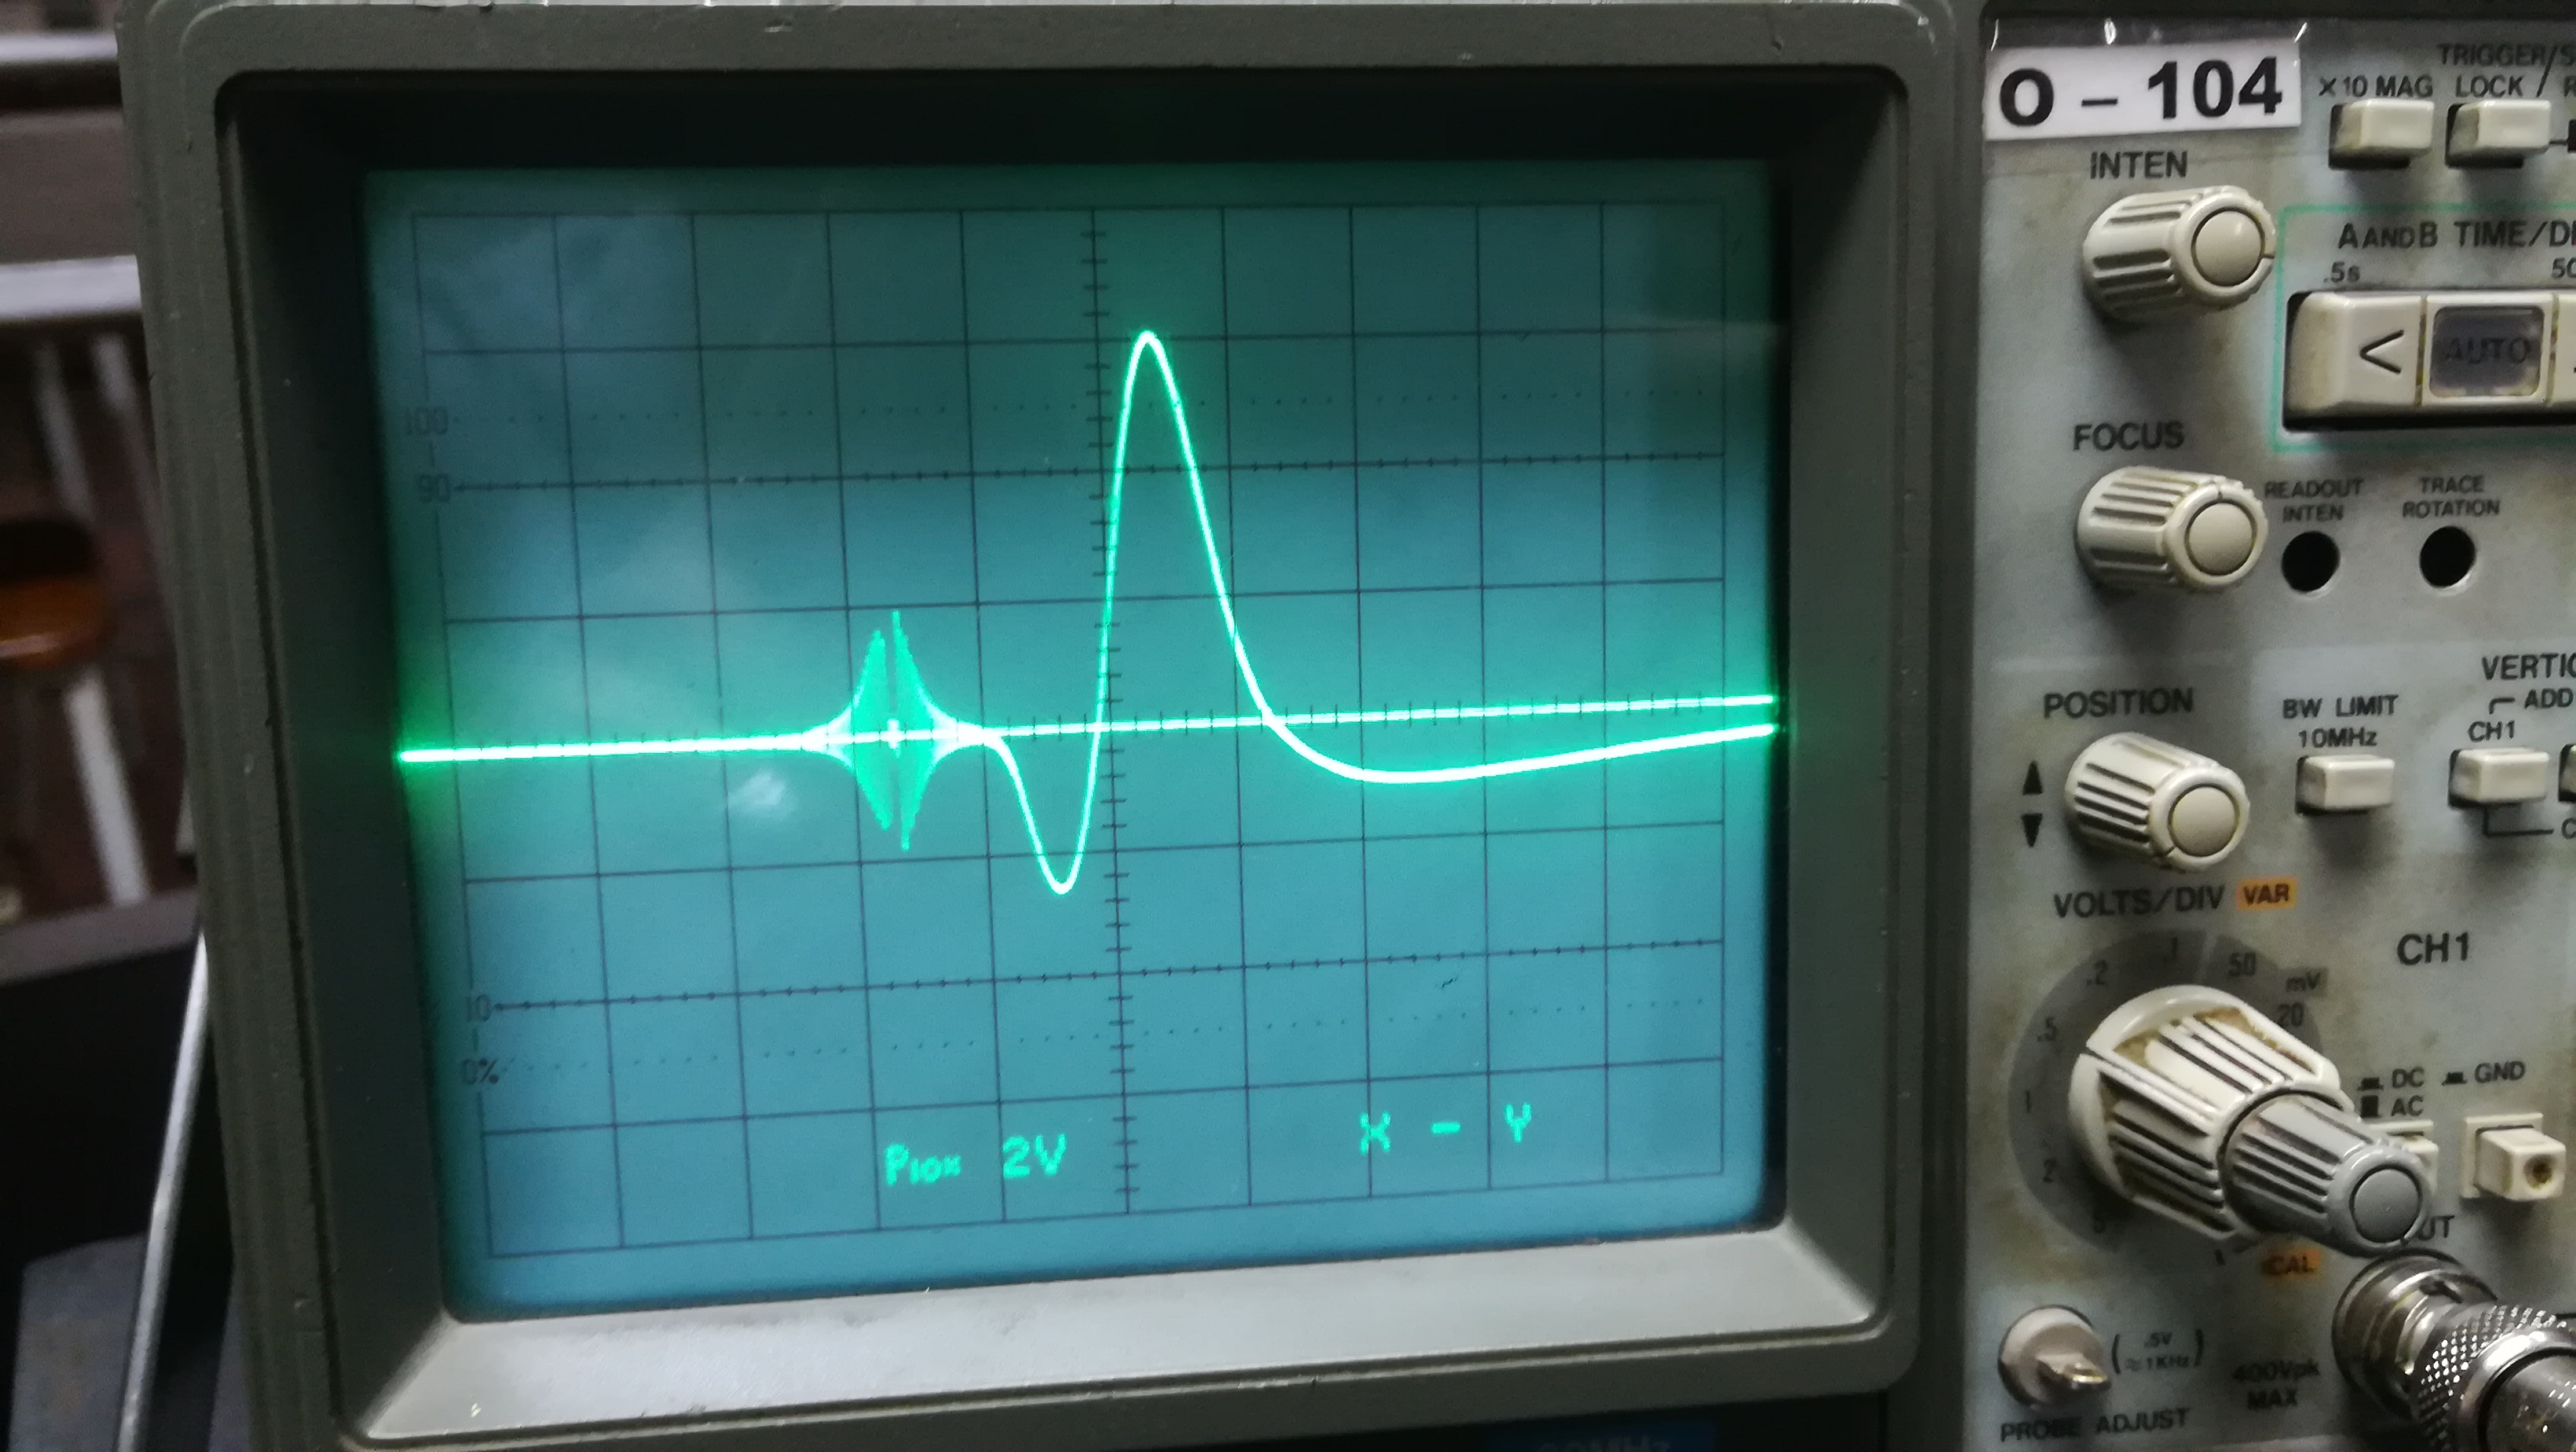
\includegraphics[width=\textwidth]{Imagenes/ActividadPractica/CaracteristicasDeDeteccion/Exp2.2_AmpliFI_MarcaAIzquierda.jpg}}
        \caption{Seteo del espectro junto con la marca.}
        \label{fig:EspectroaFI}
      \end{subfigure}

      \caption{Espectro del amplificador de FI del detector.}
      \label{fig:MediccionEspectroFIDetector}
    \end{figure}

    Ahora, se procede a la medición de la frecuencia mínima del conjunto del detector y el amplificador de FI,
    cuyo valor es $\mathbf{f_{FImin} = 10,25~MHz}$, tal y como se observa en la Figura~\ref{fig:FrecuenciaMinFI}.

    \begin{figure}[H]
      \centering
      \begin{subfigure}[ht]{0.48\textwidth}
        \frame{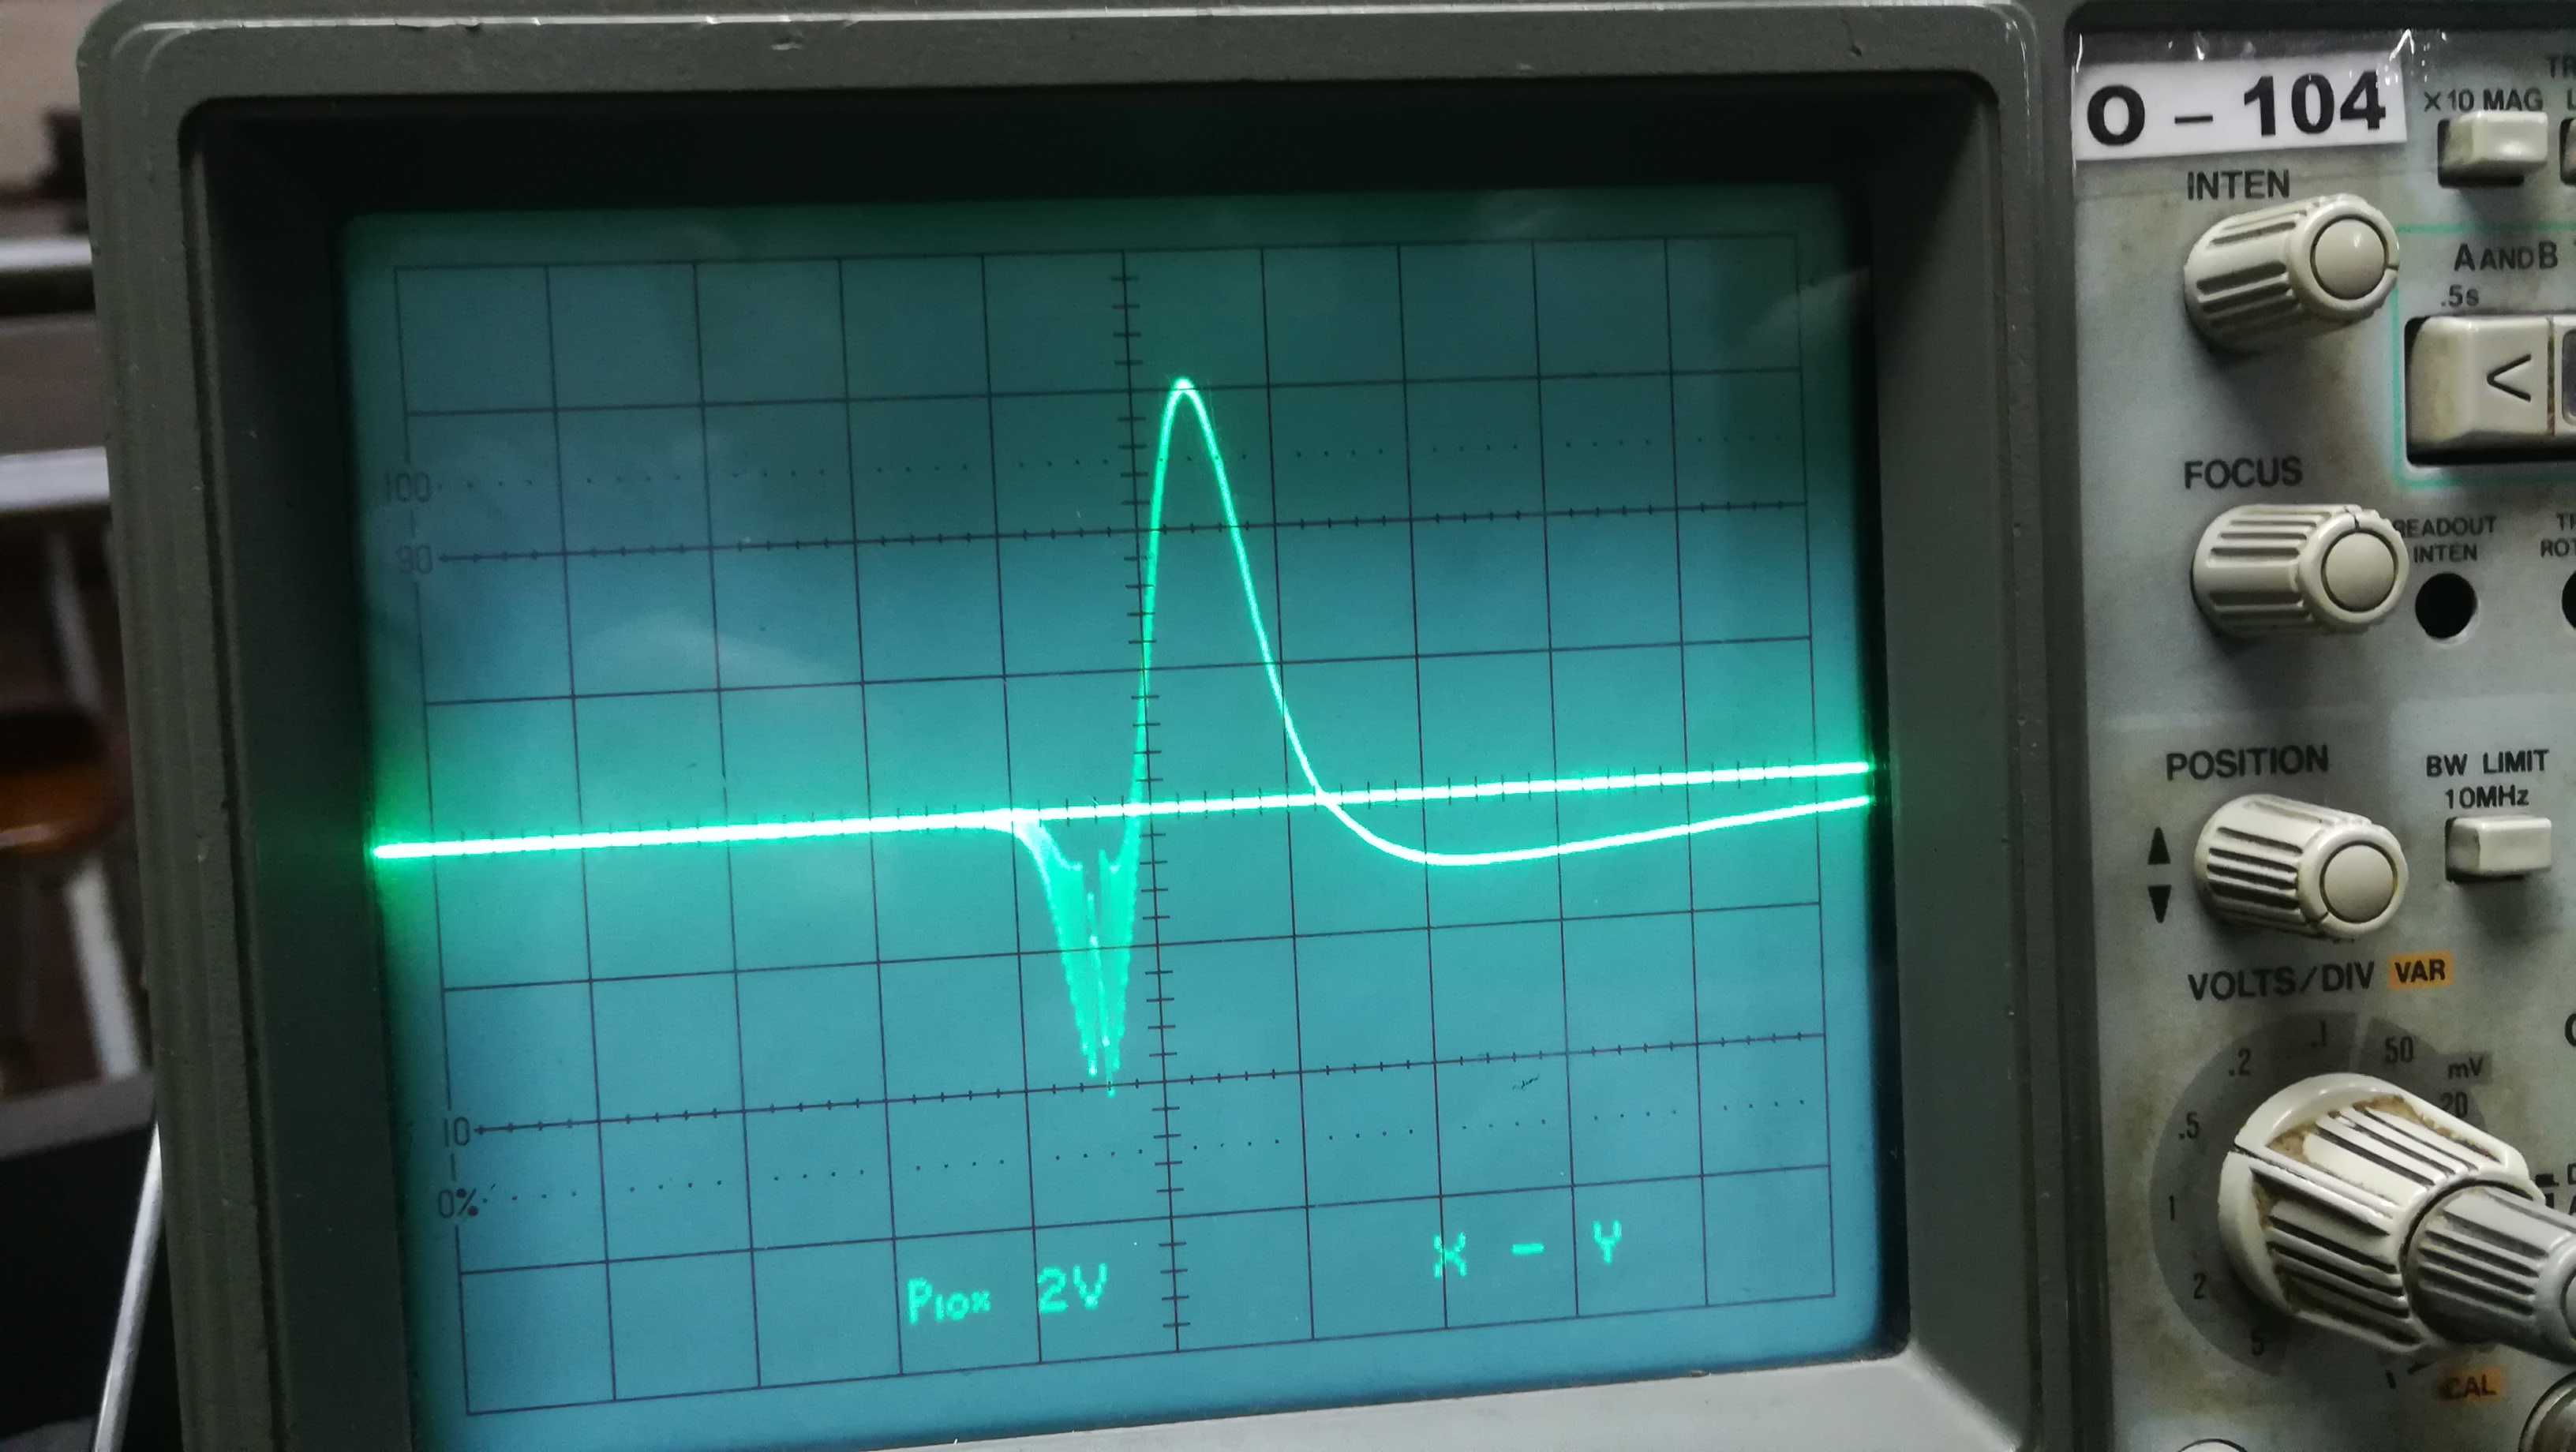
\includegraphics[width=\textwidth]{Imagenes/ActividadPractica/CaracteristicasDeDeteccion/Exp2.4_AmpliFI_FcMin.jpg}}
        \caption{Marca en la frecuencia mínima.}
        \label{fig:FrecuenciaMinFI_Osc}
      \end{subfigure}
      \hfill 
      \begin{subfigure}[ht]{0.48\textwidth}
        \frame{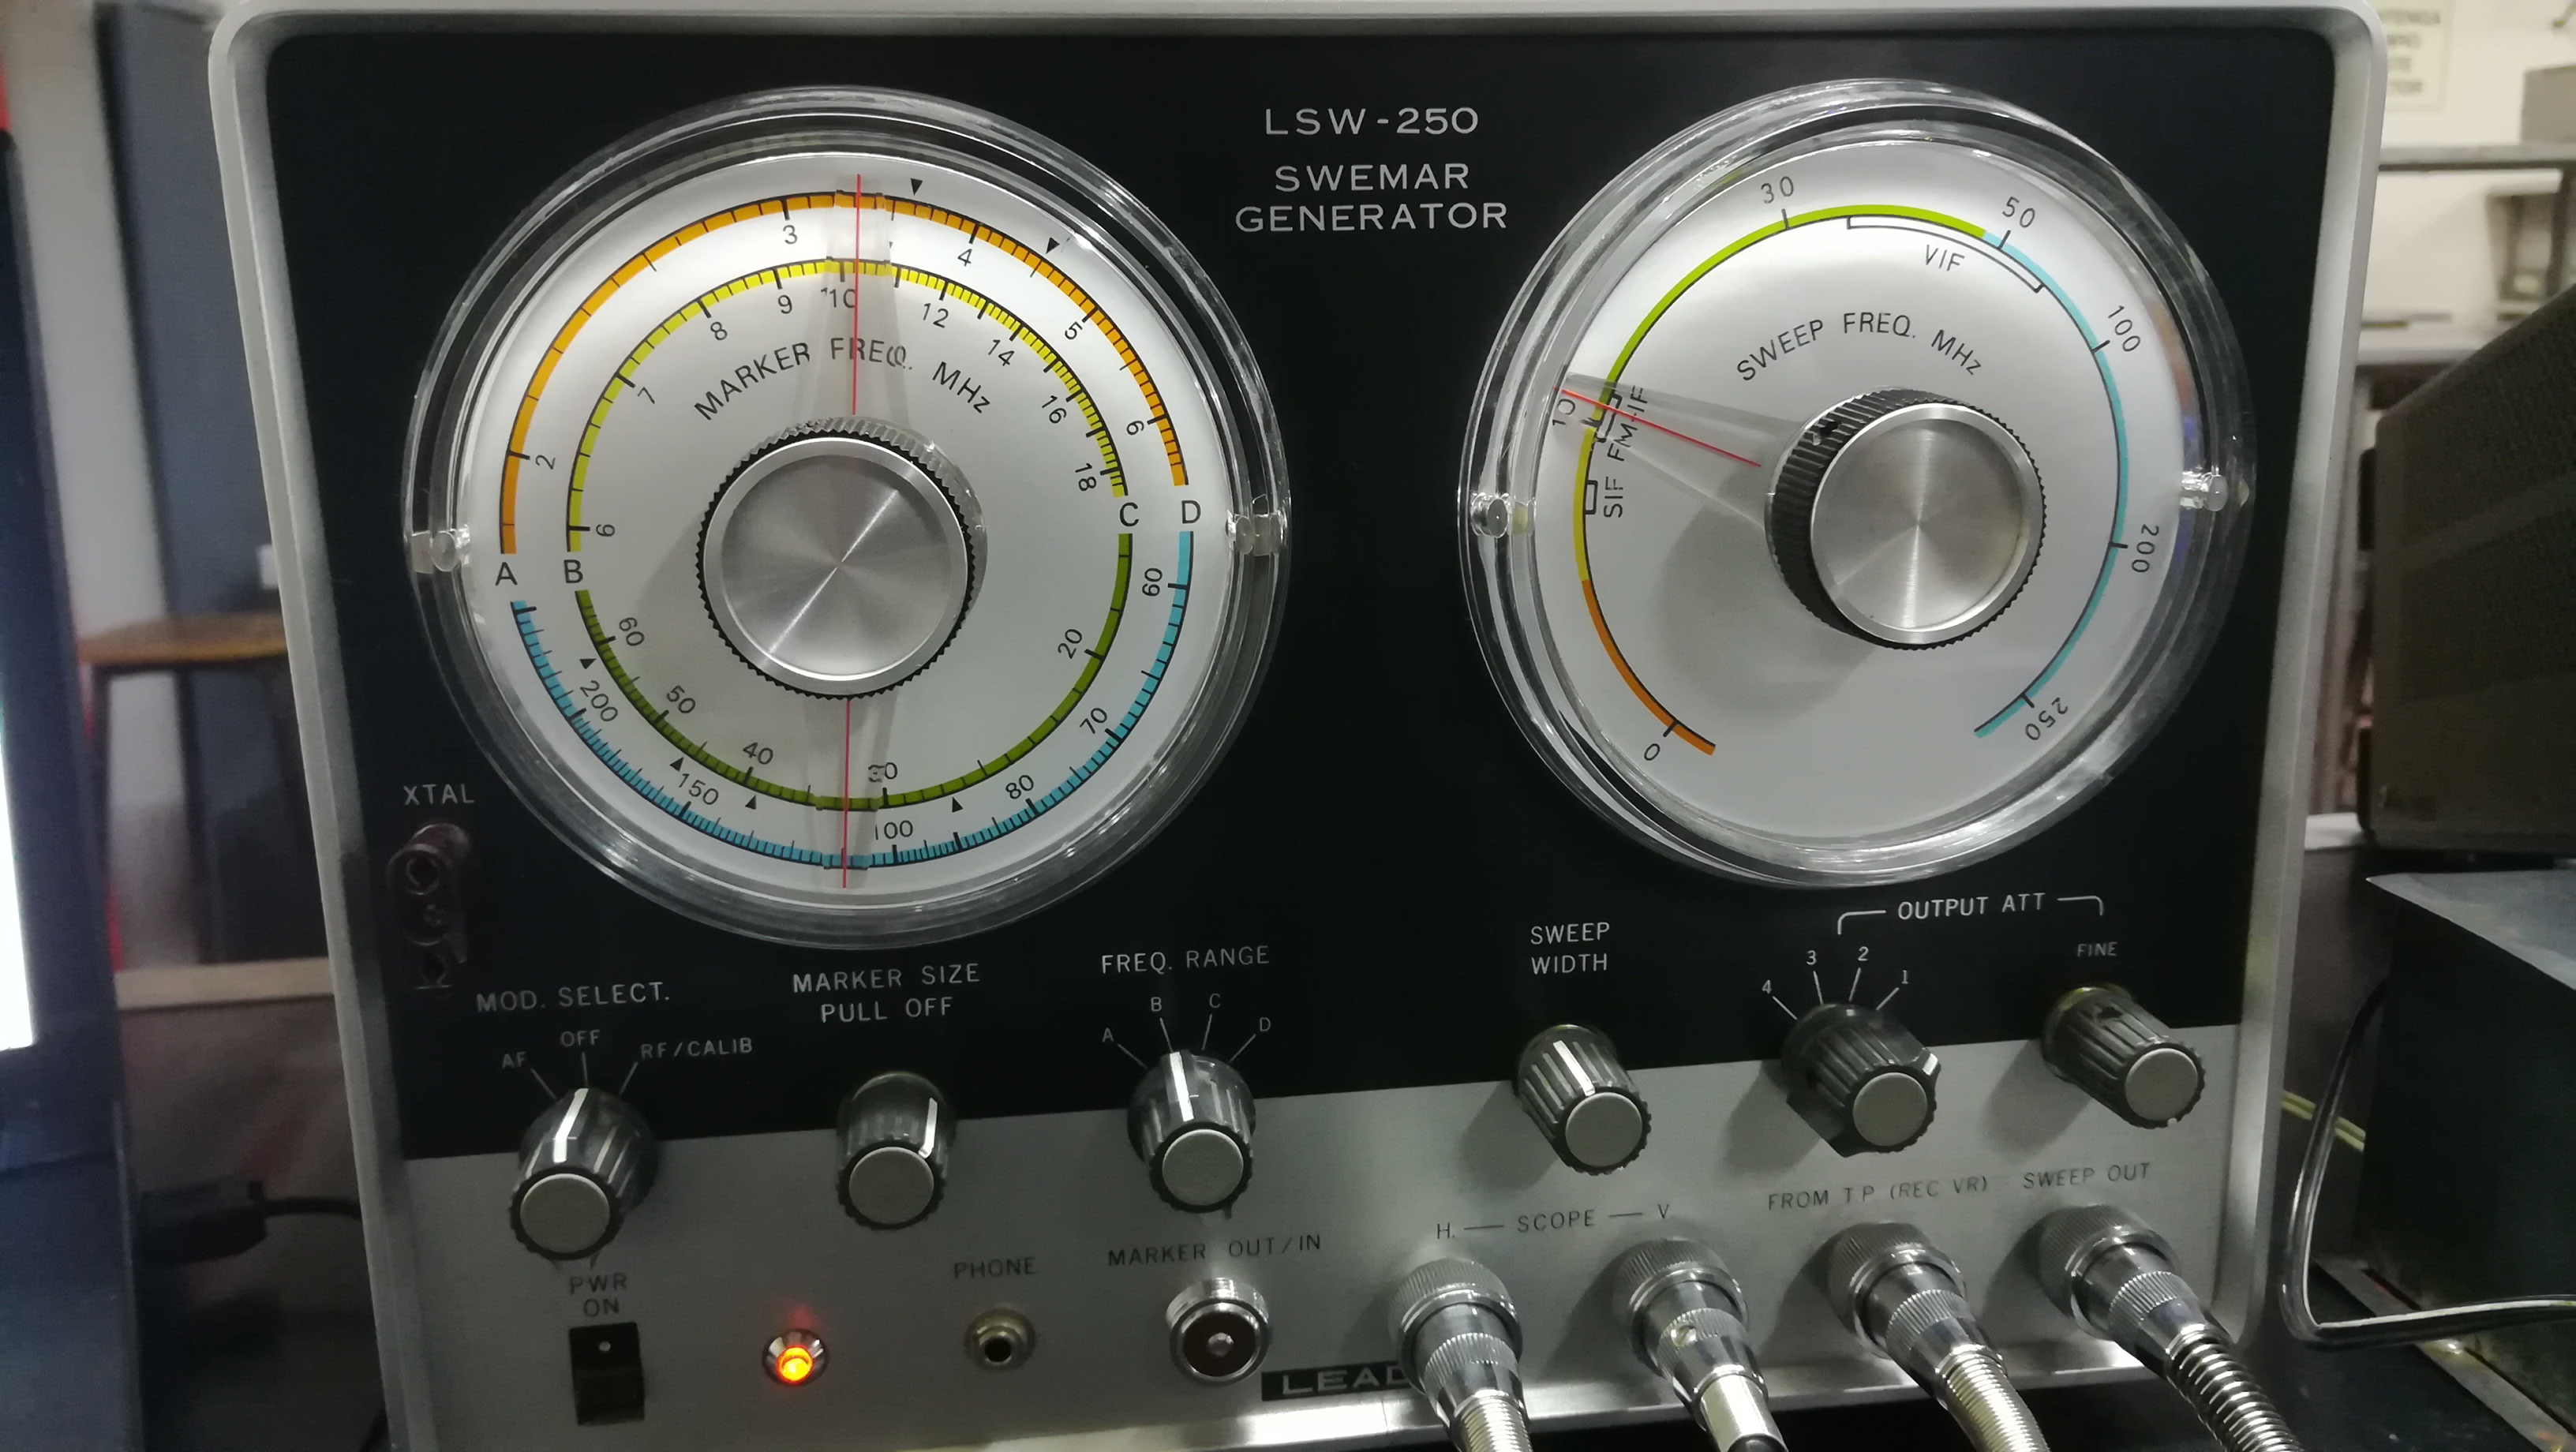
\includegraphics[width=\textwidth]{Imagenes/ActividadPractica/CaracteristicasDeDeteccion/Exp2.5_AmpliFI_FcMin_DialMarca.jpg}}
        \caption{$f_{FImin} = 10,25~MHz$.}
        \label{fig:FrecuneciaMinFI_Gener}
      \end{subfigure}

      \caption{Medición de frecuencia mínima del amplificador de FI y el detector.}
      \label{fig:FrecuenciaMinFI}
    \end{figure}

    De la misma forma, se lleva la marca a la posición central del espectro, y se mide la frecuencia central 
    del detector y el amplificador de FI. En la Figura~\ref{fig:FrecuenciaCenFI} se puede ver que dicha 
    frecuencia medida es $\mathbf{f_{FIcen} = 10,45~MHz}$.

    \begin{figure}[H]
      \centering
      \begin{subfigure}[ht]{0.48\textwidth}
        \frame{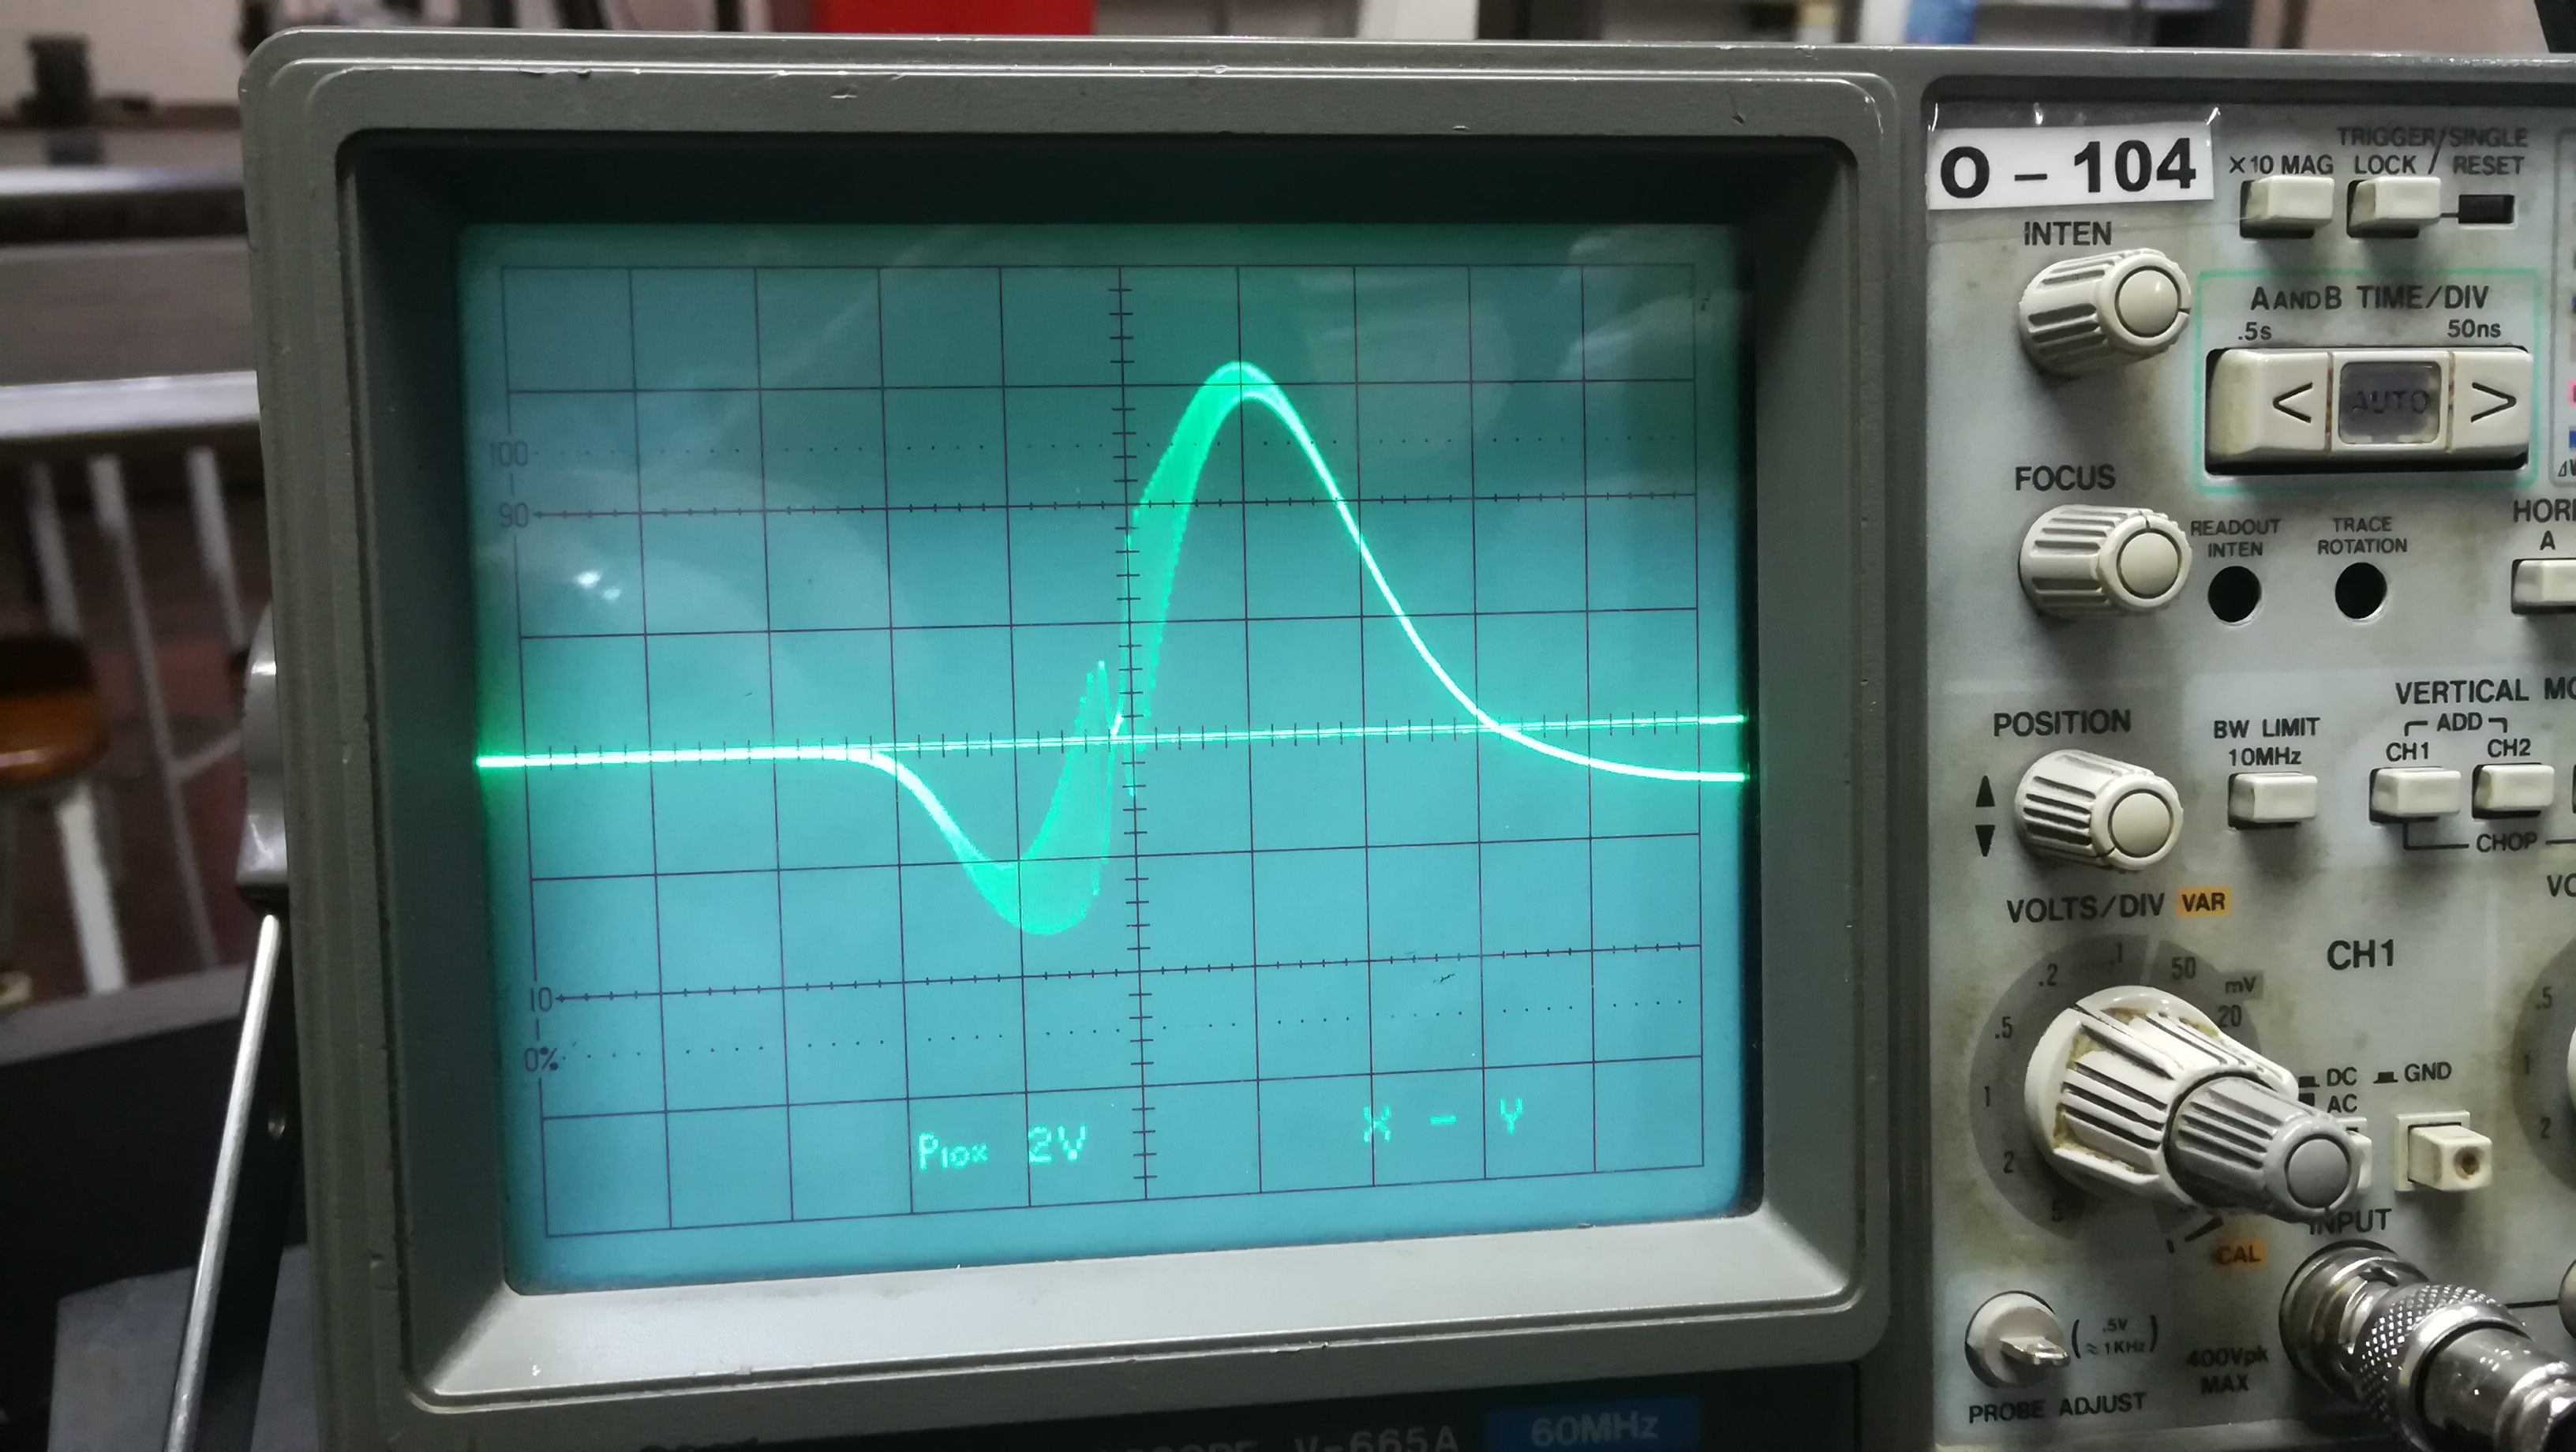
\includegraphics[width=\textwidth]{Imagenes/ActividadPractica/CaracteristicasDeDeteccion/Exp2.9_AmpliFI_FCentral.jpg}}
        \caption{Marca en la frecuencia central.}
        \label{fig:FrecuenciaCenFI_Osc}
      \end{subfigure}
      \hfill 
      \begin{subfigure}[ht]{0.48\textwidth}
        \frame{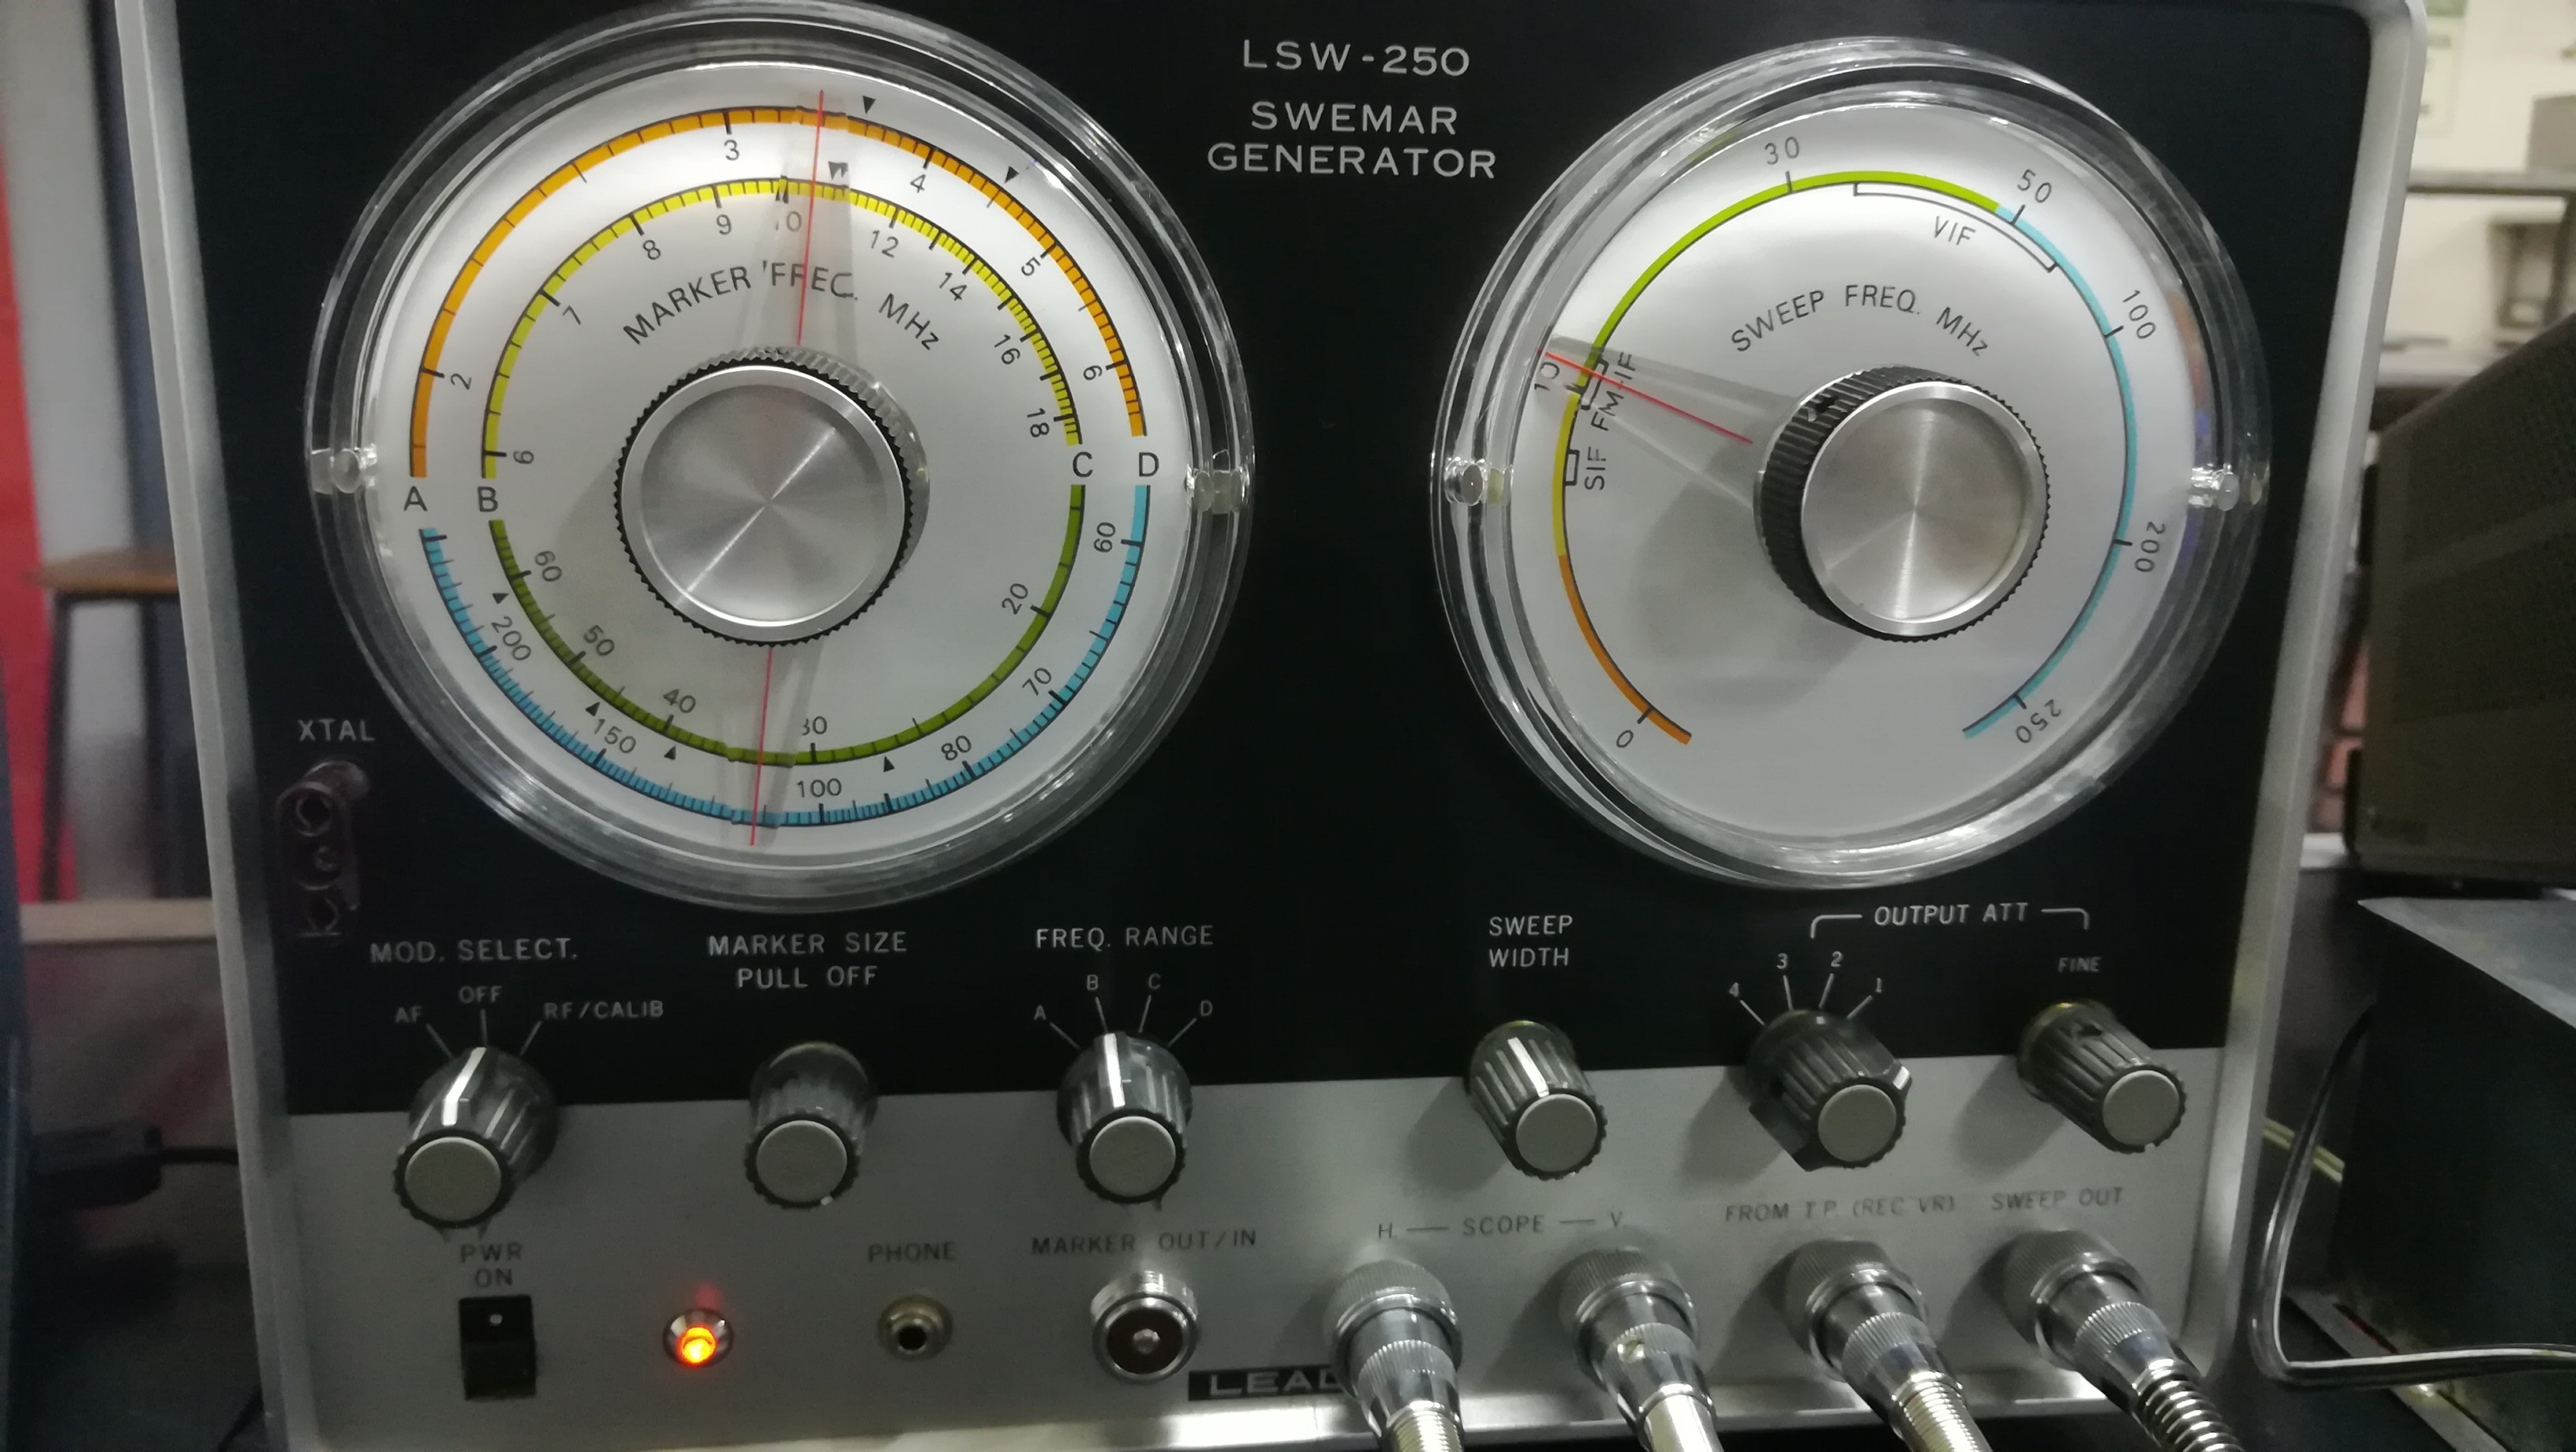
\includegraphics[width=\textwidth]{Imagenes/ActividadPractica/CaracteristicasDeDeteccion/Exp2.9_AmpliFI_FCentral_DialMarca.jpg}}
        \caption{$f_{FIcen} = 10,45~MHz$.}
        \label{fig:FrecuneciaCenFI_Gener}
      \end{subfigure}

      \caption{Medición de frecuencia central del amplificador de FI y el detector.}
      \label{fig:FrecuenciaCenFI}
    \end{figure}

    Por último, la frecuencia máxima en cuestión se puede apreciar en la Figura~\ref{fig:FrecuenciaMaxFI}, 
    la cual da un valor de $\mathbf{f_{FImax} = 10,65~MHz}$.

    \begin{figure}[H]
      \centering
      \begin{subfigure}[ht]{0.48\textwidth}
        \frame{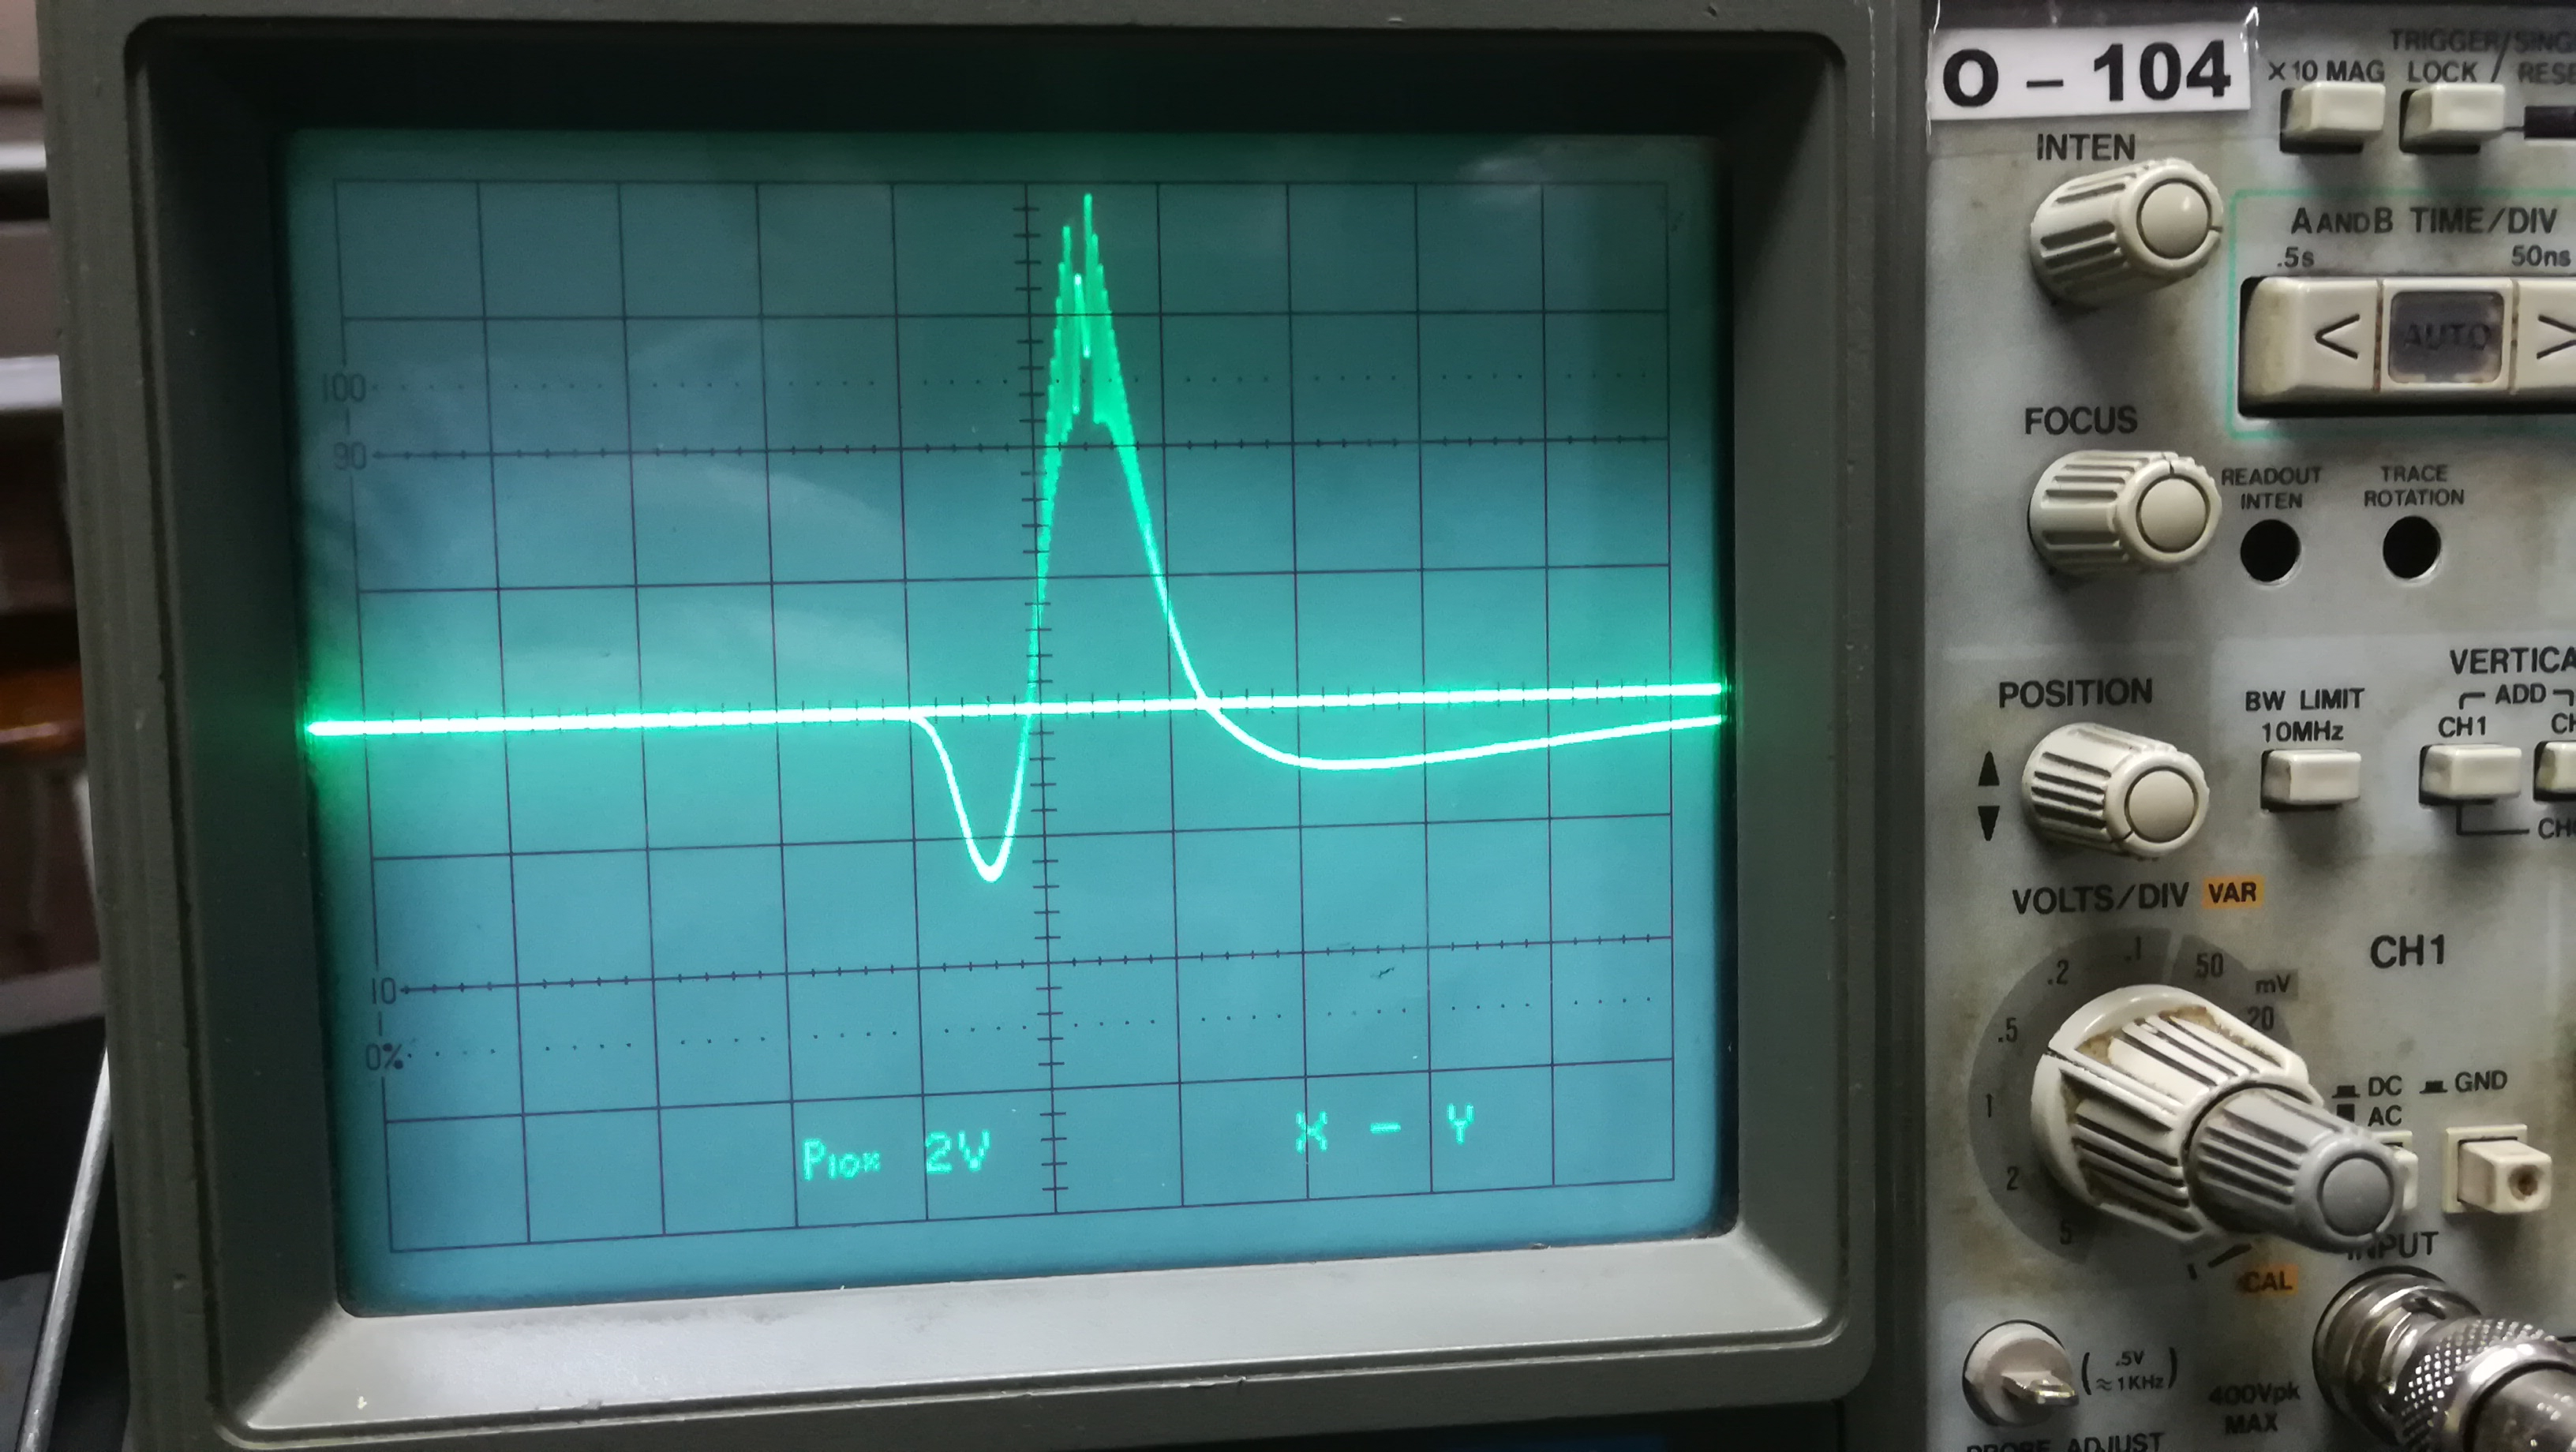
\includegraphics[width=\textwidth]{Imagenes/ActividadPractica/CaracteristicasDeDeteccion/Exp2.6_AmpliFI_FcMax.jpg}}
        \caption{Marca en la frecuencia máxima.}
        \label{fig:FrecuenciaMaxFI_Osc}
      \end{subfigure}
      \hfill 
      \begin{subfigure}[ht]{0.48\textwidth}
        \frame{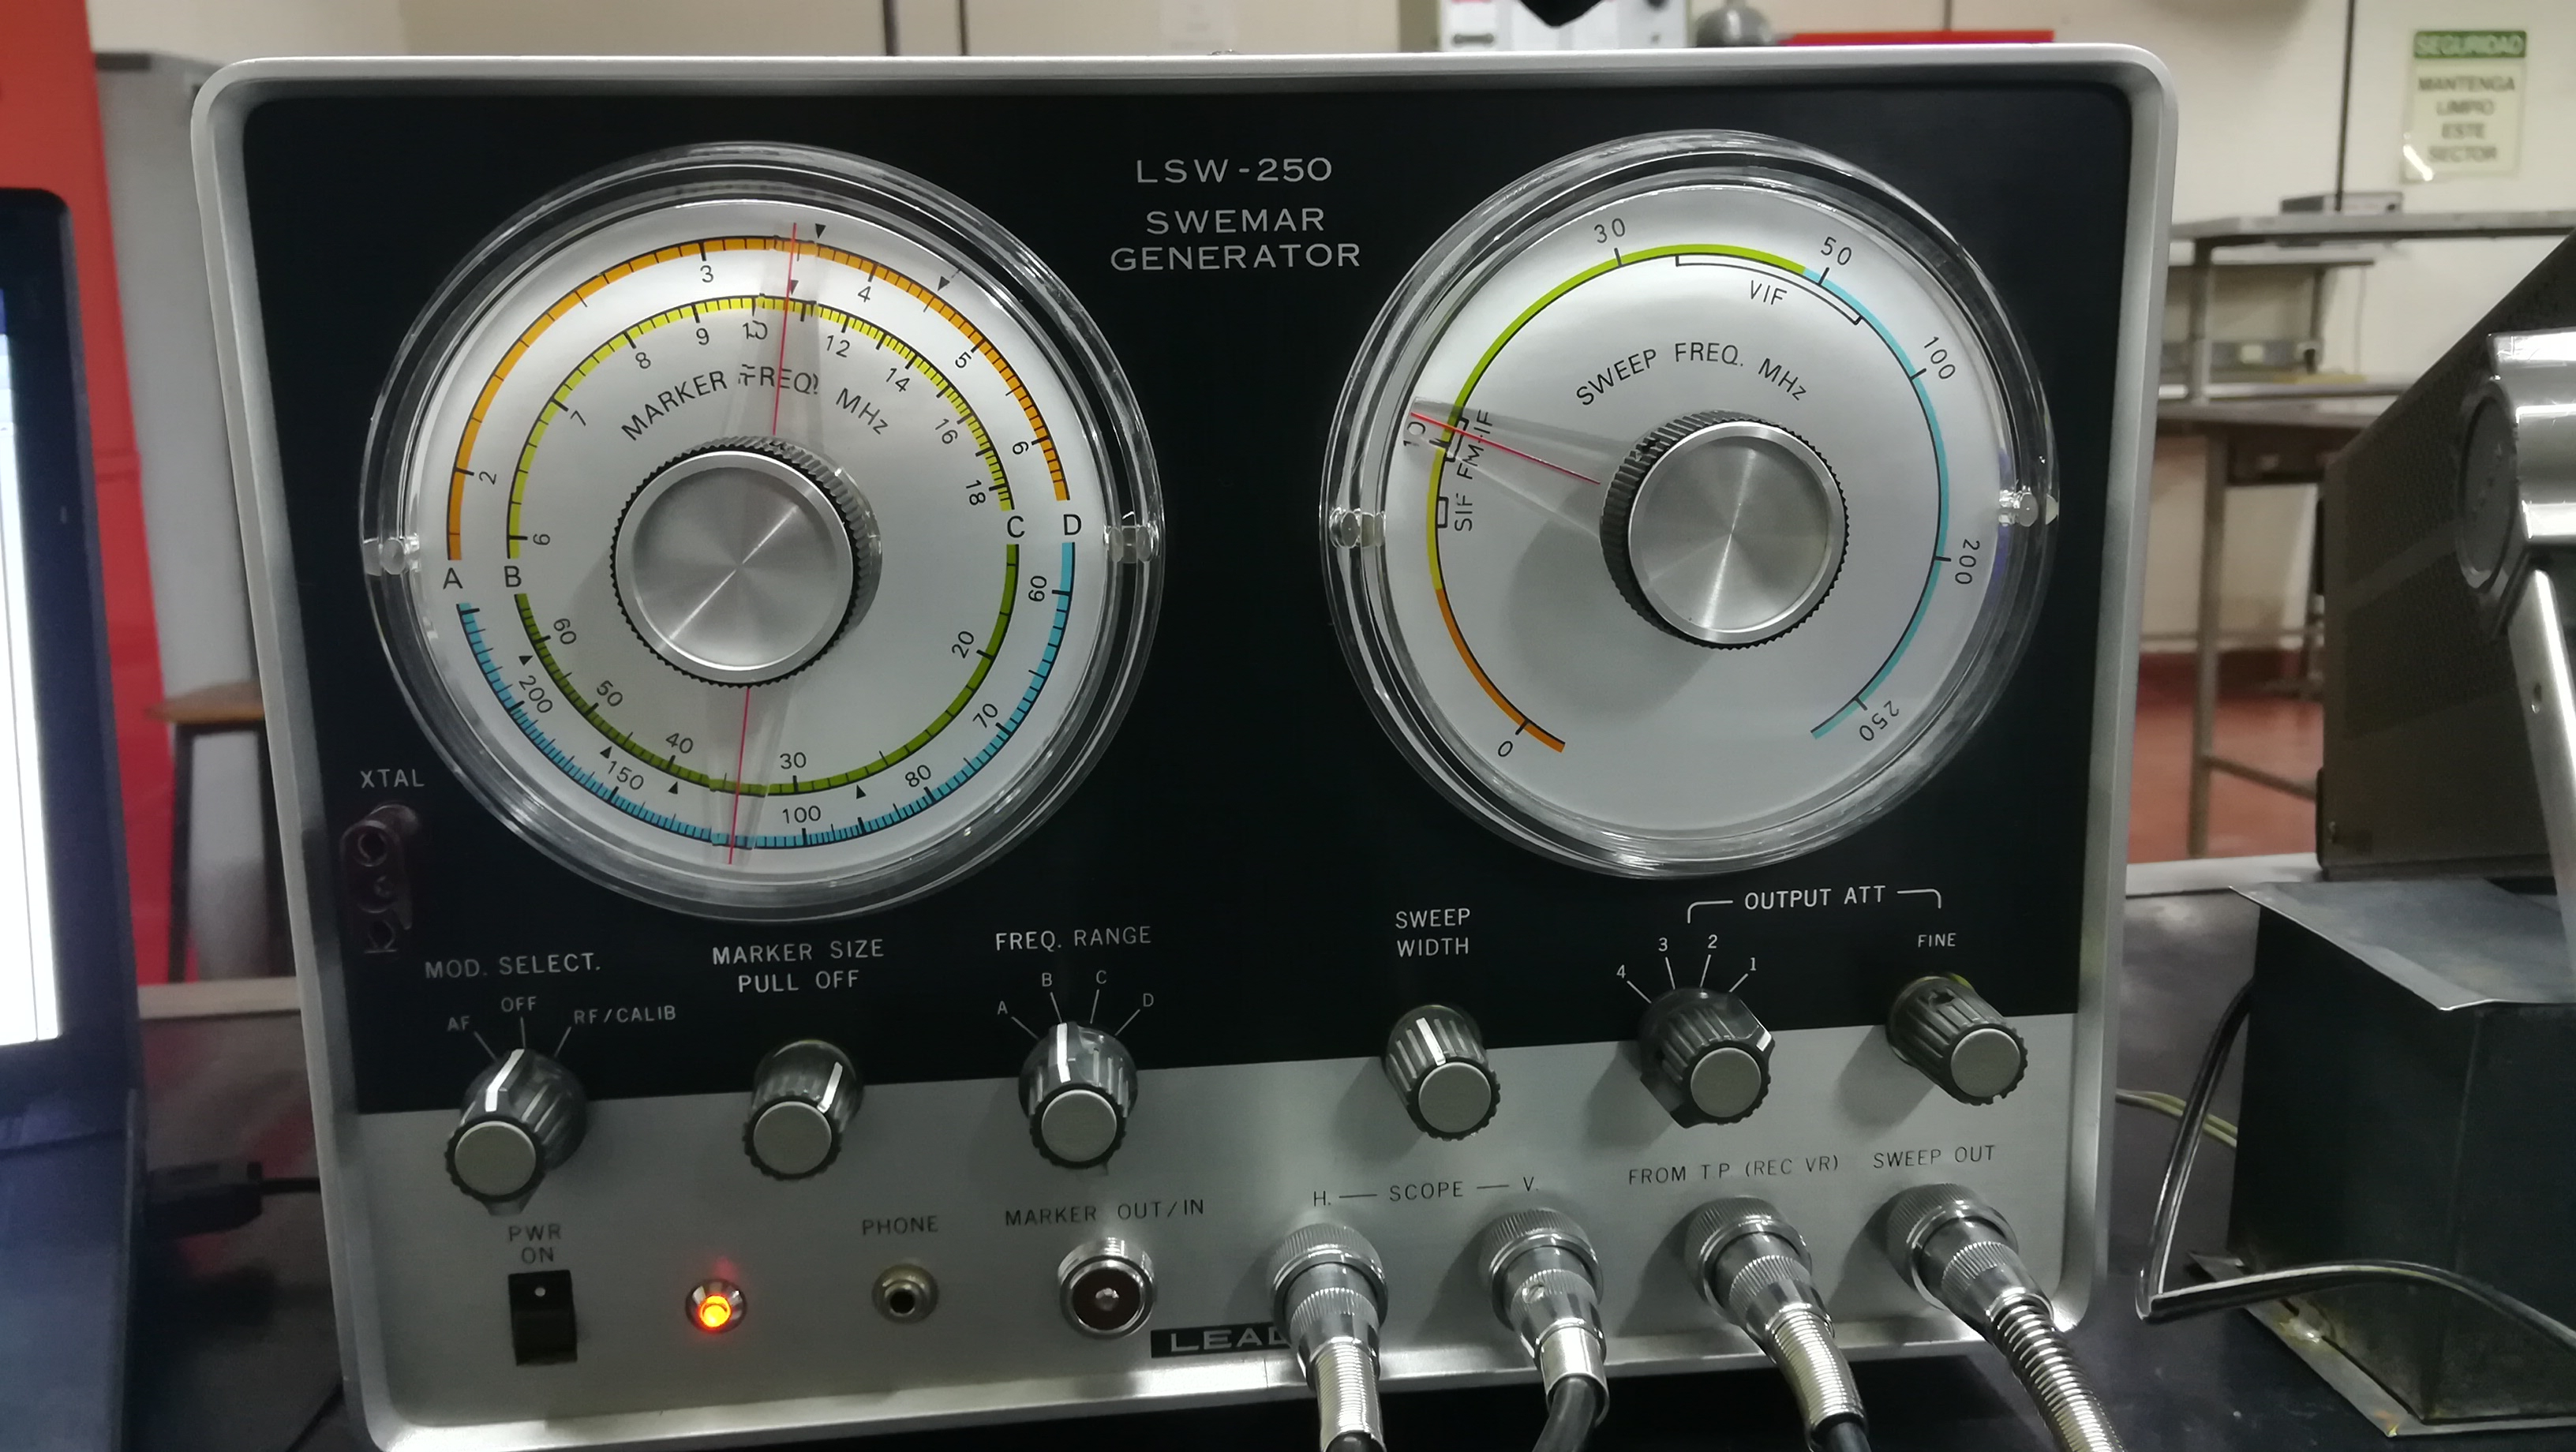
\includegraphics[width=\textwidth]{Imagenes/ActividadPractica/CaracteristicasDeDeteccion/Exp2.7_AmpliFI_FcMax_DialMarca.jpg}}
        \caption{$f_{FImax} = 10,65~MHz$.}
        \label{fig:FrecuneciaMaxFI_Gener}
      \end{subfigure}

      \caption{Medición de frecuencia máxima del amplificador de FI y el detector.}
      \label{fig:FrecuenciaMaxFI}
    \end{figure}

    Los valores obtenidos durante esta experiencia se encuentran en forma tabulada en la Tabla~\ref{tab:MedicionesFI}.

        \begin{table}[H]
            \small
            \centering
            \begin{tabular}{cccc}
                 \toprule
                 \textbf{Frec. central} $\mathbf{[MHz]}$ &  \textbf{Frec. mín.} $\mathbf{[MHz]}$ & 
                  \textbf{Frec. máx.} $\mathbf{[MHz]}$ &  $\mathbf{\triangle}$ \textbf{f} $\mathbf{[MHz]}$  \\ \midrule
                 10,45   &   10,25   & 10,65   & 0,4 \\ 
                 \bottomrule
            \end{tabular}
            \caption{Mediciones de FI obtenidas.}
            \label{tab:MedicionesFI}
        \end{table}
